\chapter{LoRaWAN}
\label{chap:lorawan}

This chapter describes the LoRaWAN network protocol which is optimized for battery-powered end-devices.

LoRaWAN networks typically are laid out in a star-of-stars topology in which gateways relay messages between end-devices and a central network server at the backend. Gateways are connected to the network server via standard IP connections while end-devices use single-hop LoRa or FSK communication to one or many gateways. All communication is generally bi-directional, although uplink communication from an end-device to the network server is expected to be the predominant traffic.

%LoRaWAN networks are organized in a star-of-stars topology, in which a central network server is in charge of managing all LoRa end-devices, receiving via standard IP connections

\begin{figure}[h!]
\centering
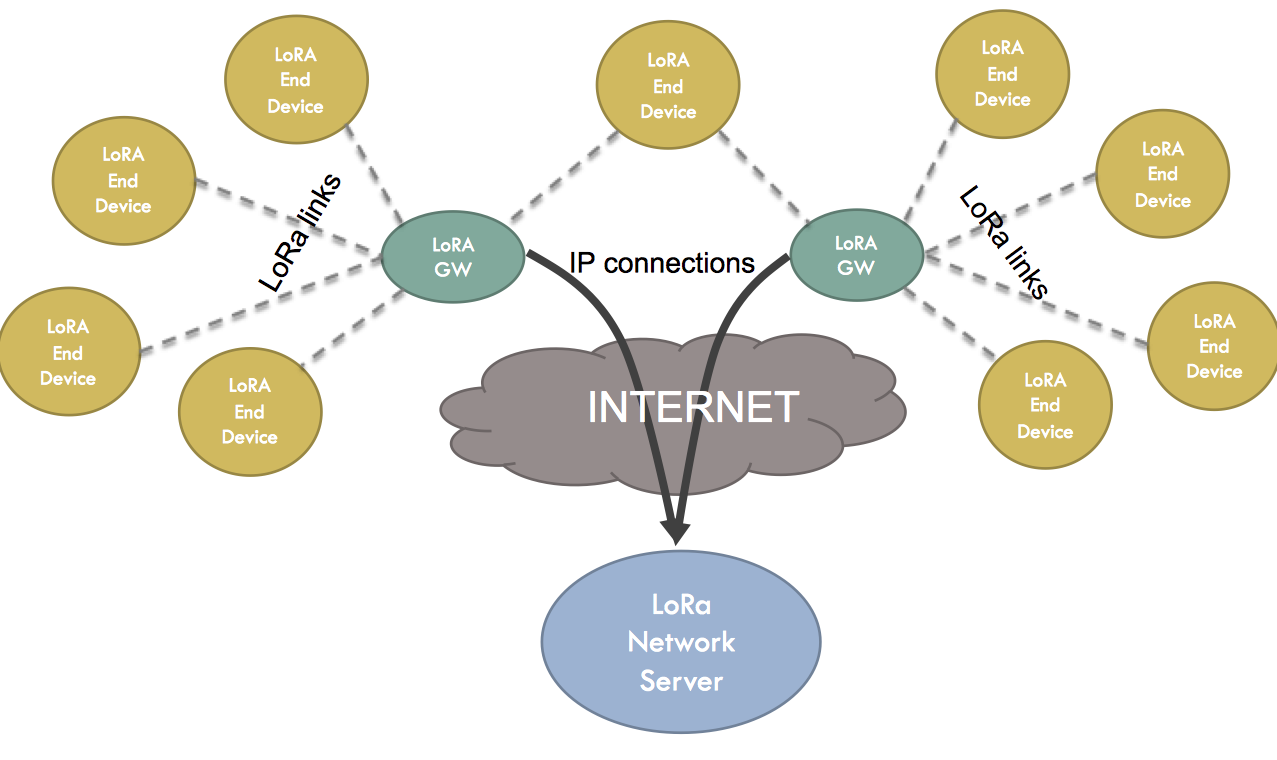
\includegraphics[width=\textwidth]{img/lora-arch}
\caption{Architecture}
\end{figure}

Communication between end-devices and gateways is spread out on different frequency channels and data rates. The selection of the data rate is a trade-off between communication range and message duration, communications with different data rates do not interfere with each other. LoRa data rates range from 0.3 kbps to 50 kbps. To maximize both battery life of the end-devices and overall network capacity, the LoRa network infrastructure can manage the data rate and RF output for each end-device individually by means of an adaptive data rate (ADR) scheme. \cite{lorawanspec}

\section{Specification}

\subsection{LoRaWAN classes}
LoRaWAN defines three classes of operation, of which only \emph{Class A} must be mandatorily implemented on all LoRaWAN compatible devices. Thanks to this policy we have a basic set of features which are present on all LoRaWAN end-devices, keeping both the architectural complexity and the production cost as low as possible.

In addition to the basic class, two more complex modes of operation has been defined with the aim to decouple downstream transmissions from the upstream ones. Given that these two advanced modes may be more expensive to design, produce and maintain, only end-devices who strongly requires these features are required to implement it.

\subsubsection{Class A: bi-directional end-devices}
In Class A communications each end-device's uplink transmission is followed by two short downlink receive windows. Each end-device schedules the transmission slots depending on its own needs, as in a ALOHA-type of protocol.

The main advantage of this communication scheme is the very low power consumption, while the biggest drawback is that this class of operation is suitable only for applications which allow to receive data only after the end-device has sent an uplink transmission. In fact downlink communications from the server at any other time will have to wait until the next scheduled uplink.


\subsubsection{Class B: bi-directional end-devices with scheduled receive slots}
In order to overcome the problem of non-deterministic latency on downlink communications, Class B increases the number of receive windows opened by the end-devices. These extra receive windows are synchronized with the server by means of a time-stamped beacon, which is broadcast by the gateway.


\subsubsection{Class C: bi-directional end-devices with maximal receive slots}
To offer the lowest possible latency to the server for downlink communication, Class C end-devices have a continuously open receive windows, which is closed only when transmitting data. This better performances are offered at the cost of an higher power consumption than Class A and B.

\subsection{Class A receive windows}
Following each uplink transmission the end-device opens two short receive windows. The receive window starts exactly after a predefined interval of time from the transmission of the last uplink bit. \cite{lorawanspec}

\begin{figure}[h!]
\centering
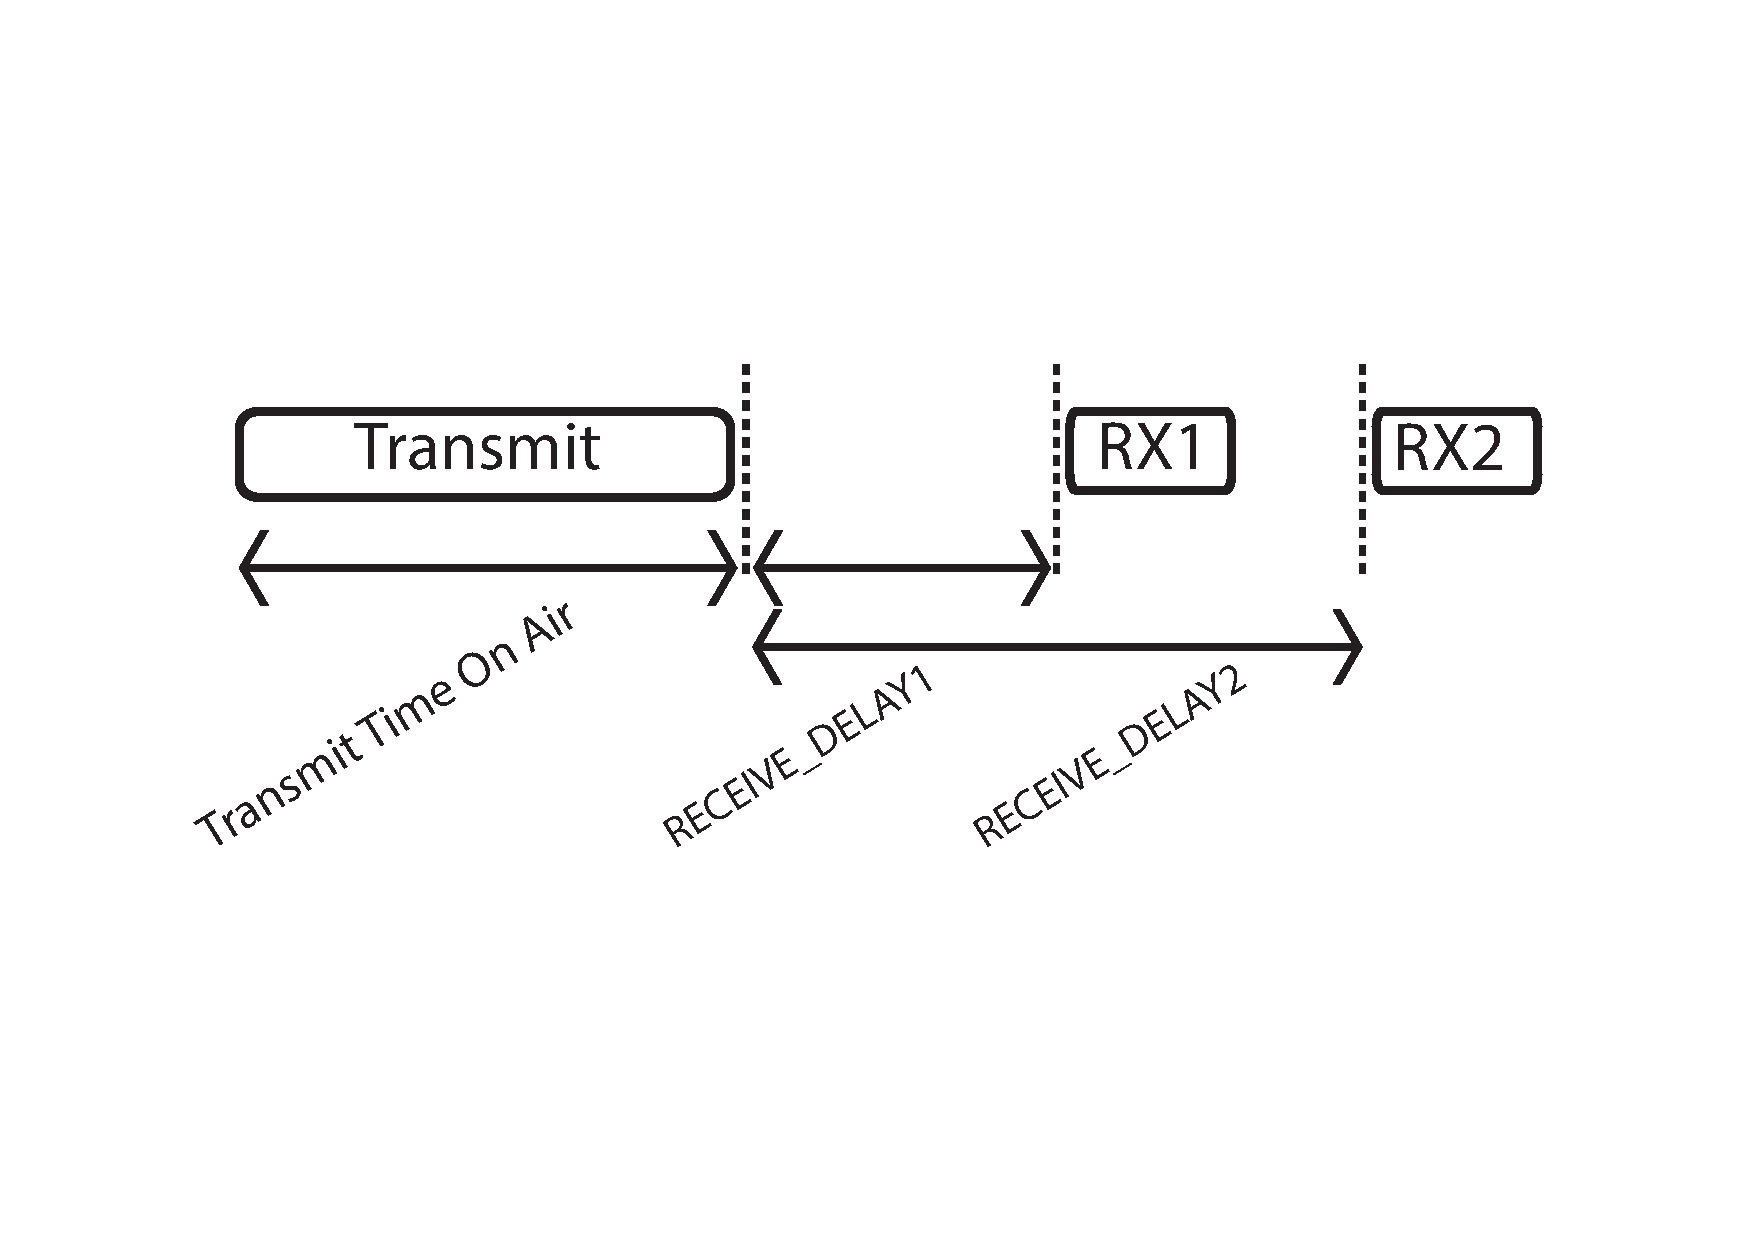
\includegraphics[width=\textwidth]{img/recwin}
\caption{LoRaWAN receive windows}
\end{figure}


The first receive window (RX1) is opened after RECEIVE\_DELAY1 milliseconds, which by default is set to 1 second. It uses the same frequency as the previous uplink transmission, and in general also the same data rate (in some regions may be a function of the uplink data rate).

The second receive window (RX2) is opened after RECEIVE\_DELAY2 milliseconds, which is defined as RECEIVE\_DELAY1 + 1 second. The frequency and the data rate are fixed for all transmissions, which means that they do not depend on the previous uplink communication, and they are configurable through a MAC command (table \ref{tab:cmd1}).

Each receive window is kept open at least for the time required to detect preamble of a LoRa downlink transmission, which is in the order of microseconds. If a frame is correctly received during the first receive window, the end-device does not open the second one. An end-device shall not transmit an other uplink message before a downlink message is received or the RX2 window is expired.


\subsection{Message Format}
LoRaWAN provides a full stack network protocol, having features of data-link, network and transport layer, and natively supporting encryption, authentication and reliable communication trough packet retransmission.

\subsubsection{Radio physical layer}

Each LoRa packet carries a physical payload (\emph{PHYPayload}) which contains LoRaWAN messages. When a LoRa packet contains a LoRaWAN message the CRC field, calculated on PHYPayload, is present only in up-link transmissions, since it is disabled for down-link transmissions.

\begin{figure}[h!]
\centering
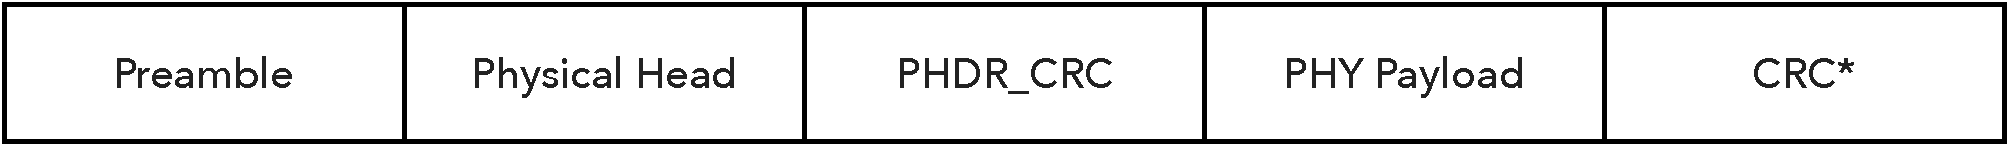
\includegraphics[width=\textwidth]{img/msgformat/radio}
\caption{LoRa radio physical layer (CRC only uplink messages)}
\end{figure}


\subsubsection{Physical payload}

The physical payload contains three main fields:

\begin{itemize}

\item \emph{MAC Header}: specifies the \emph{Message Type} and the \emph{version} of LoRaWAN;

\item \emph{MAC Payload}: contains the LoRaWAN Frame;

\item \emph{MIC}: the Message Integrity Code, it is calculated as specified in RFC 4493 and it authenticates each message to the LoRa Network Server.

$MIC = aes128_cmac(NetSessionKey, B0 | msg) [0...3]$

\end{itemize}

\begin{figure}[h!]
\centering
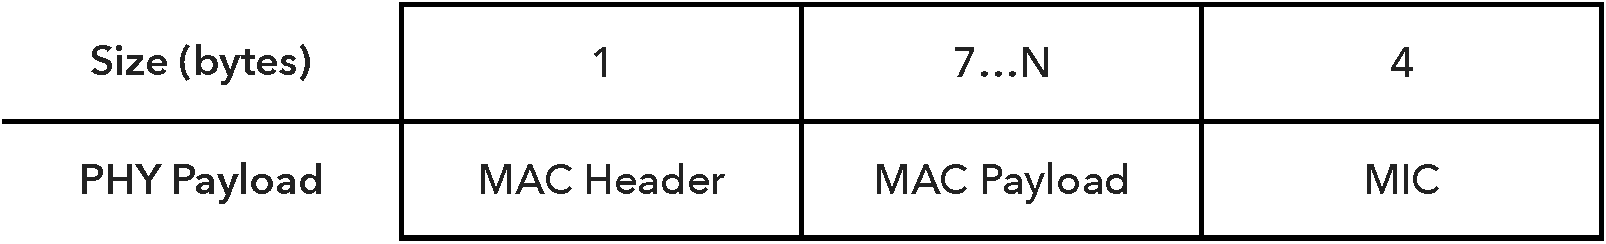
\includegraphics[width=\textwidth]{img/msgformat/phy_payload}
\caption{LoRa physical payload structured as a LoRaWAN message}
\end{figure}


\subsubsection{MAC Header}
The MAC header specifies the \emph{Message Type} and the \emph{version} of LoRaWAN. In table \ref{tab:msgtypes} all possible LoRaWAN message types are reported.


\begin{figure}[h!]
\centering
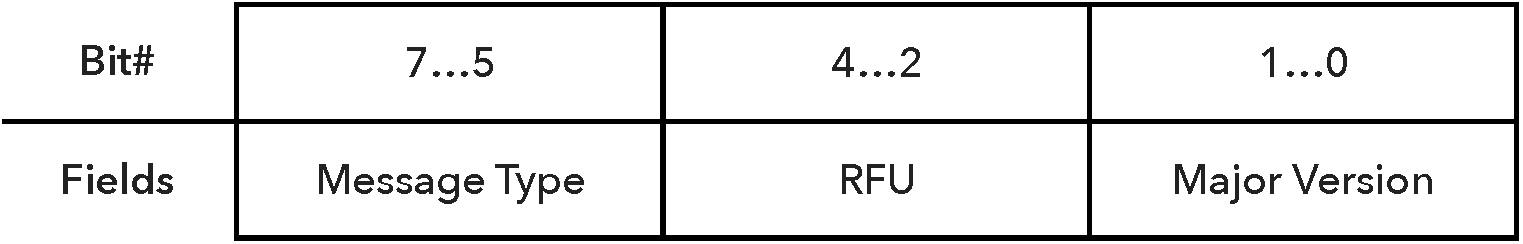
\includegraphics[width=\textwidth]{img/msgformat/mac_header}
\caption{LoRaWAN MAC header}
\end{figure}




% Please add the following required packages to your document preamble:
% \usepackage{booktabs}
\begin{table}[h!]
\centering
\caption{LoRaWAN message types}
\label{tab:msgtypes}
\begin{tabular}{@{}ll@{}}
\toprule
Msg Type & Description          \\ \midrule
000          & Join Request          \\
001          & Join Accept           \\
010          & Unconfirmed Data Up   \\
011          & Unconfirmed Data Down \\
100          & Confirmed Data Up     \\
101          & Confirmed Data Down   \\
110          & RFU                   \\
111          & Proprietary           \\ \bottomrule
\end{tabular}
\end{table}


\subsubsection{MAC Payload}
The MAC payload contains mandatory \emph{Frame Header} fields and optionally \emph{Frame Port} and \emph{Frame Payload}. Frame


\begin{figure}[h!]
\centering
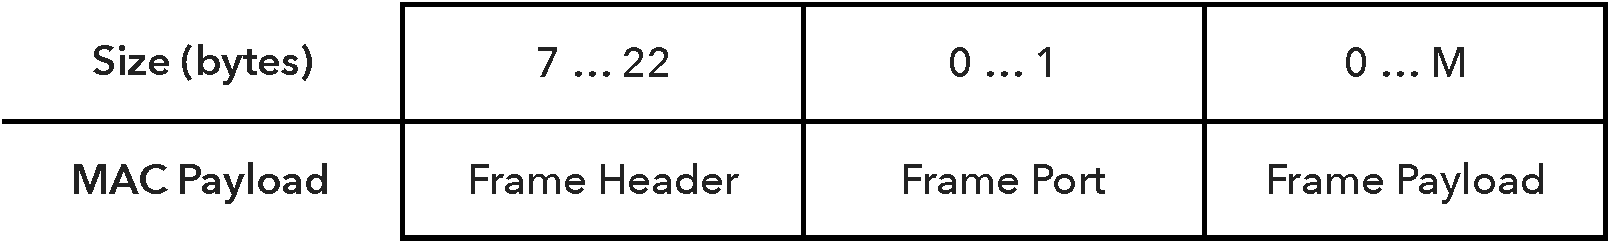
\includegraphics[width=\textwidth]{img/msgformat/mac_payload}
\caption{LoRaWAN MAC payload}
\end{figure}


\subsubsection{Frame Header}
The \emph{Frame Header} contains the 32 bit \emph{Device Address}, the \emph{Frame Control} field, the \emph{Frame Counter} and the \emph{Frame Options} field, which is used to piggyback MAC commands on user data traffic.

\begin{figure}[h!]
\centering
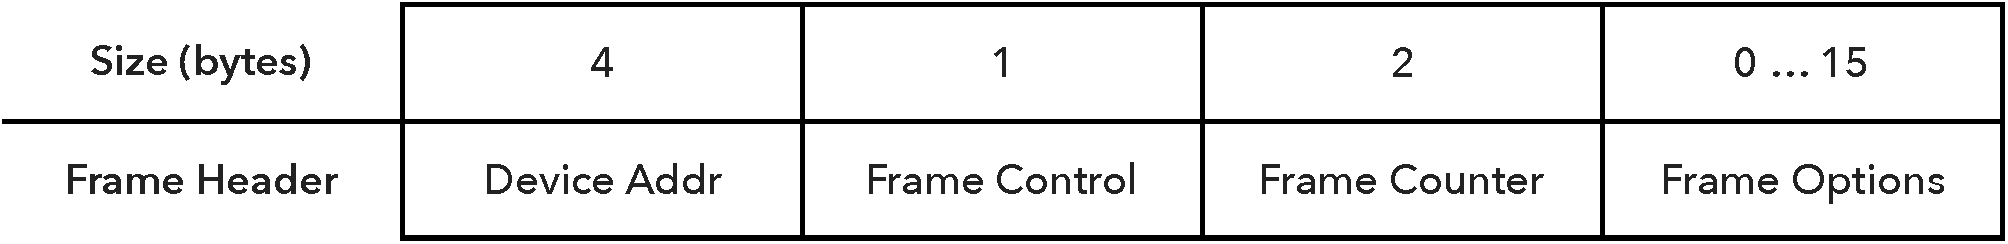
\includegraphics[width=\textwidth]{img/msgformat/frame_header}
\caption{LoRaWAN frame header}
\end{figure}

In the \emph{Frame Control} there are several important flags: the \emph{ADR} flag signals that data rate is controlled by network; the \emph{ADRACKReq} is set by the device to check if the gateway is still able to receive its traffic; the \emph{ACK} flag is set to acknowledge the previous received packet.

\begin{figure}[h!]
\centering
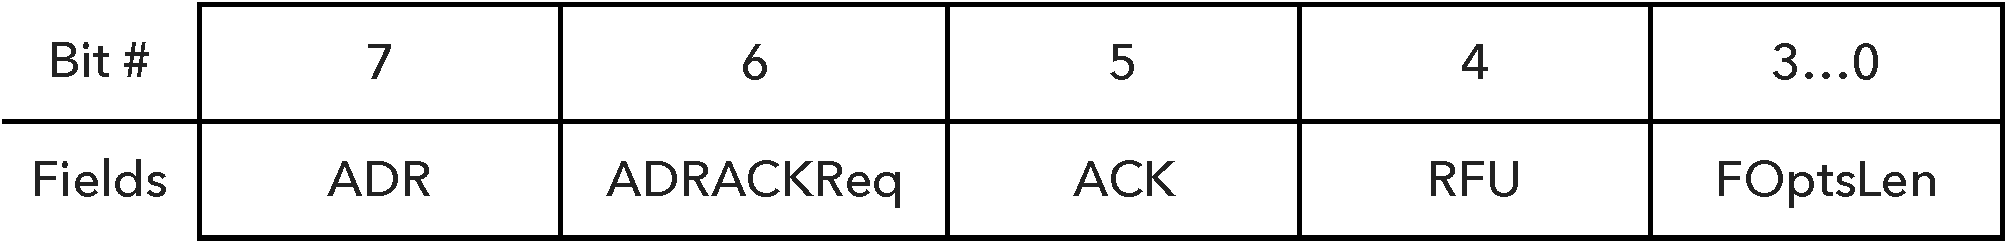
\includegraphics[width=\textwidth]{img/msgformat/frame_control}
\caption{LoRaWAN frame control}
\end{figure}


\subsubsection{Frame Port and Frame Payload}
By default LoRaWAN encrypts every Frame Payload by means of the \emph{Application Session Key}. If the Frame Payload carries a MAC command, then the Frame Port is set to 0 and it is encrypted with \emph{Network Session Key}.
If encryption is done above the LoRaWAN layer is possible to disable this features through a MAC command, but it is allowed only if the frame payload does not carry a MAC command itself.



\subsection{MAC Commands}
The MAC commands are a set of messages exchanged exclusively between the MAC layer of the end-devices and the network server. This messages may contain information useful for network administration purposes, such as checking the status of a device or changing some communication parameters, and they are never visible to the application server running in the cloud or the application running on the end-device.

MAC commands can be sent as Frame Payload, setting Frame Port to 0 and performing the encryption by means of the NetworkSessionKey. MAC commands can be also piggybacked in the FOpts field, and in this case they must not exceed 15 octets and they are sent always in clear.

A MAC command consists of a command identifier (CID) of 1 octet followed by a possibly empty command-specific sequence of octets. CIDs in the interval between 0x00 and 0x7F are reserved, while CIDs starting from 0x80 to 0xFF are available for proprietary network extensions.

Tables \ref{tab:cmd1} and \ref{tab:cmd2} contain the list of MAC commands defined in the LoRaWAN 1.0 specification.

% Please add the following required packages to your document preamble:
% \usepackage{multirow}
\begin{table}[]
\centering
\caption{MAC commands from 0x02 to 0x05}
\label{tab:cmd1}
\begin{tabular}{ccccl}
\hline
\multirow{2}{*}{CID} & \multirow{2}{*}{Command} & \multicolumn{2}{c}{TX by} & \multicolumn{1}{c}{\multirow{2}{*}{Description}}                                                                                                                                                       \\
                     &                          & ED               & GW              & \multicolumn{1}{c}{}                                                                                                                                                                                   \\ \hline
0x02                 & LinkCheckReq             & x                &                 & \begin{tabular}[c]{@{}l@{}}Used by an end-device to \\ validate its connectivity to\\ a network.\end{tabular}                                                                                          \\
0x02                 & LinkCheckAns             &                  & x               & \begin{tabular}[c]{@{}l@{}}Answer to LinkCheckReq\\ command. Contains the \\ received signal power\\ estimation indicating to the\\ end-device the quality of \\ reception (link margin).\end{tabular} \\
0x03                 & LinkADRReq               &                  & x               & \begin{tabular}[c]{@{}l@{}}Requests the end-device to \\ change data rate, transmit \\ power, repetition rate or\\ channel.\end{tabular}                                                               \\
0x03                 & LinkADRAns               & x                &                 & \begin{tabular}[c]{@{}l@{}}Acknowledges the \\ LinkRateReq.\end{tabular}                                                                                                                               \\
0x04                 & DutyCycleReq             &                  & x               & \begin{tabular}[c]{@{}l@{}}Sets the maximum \\ aggregated transmit duty-\\ cycle of a device\end{tabular}                                                                                              \\
0x04                 & DutyCycleAns             & x                &                 & \begin{tabular}[c]{@{}l@{}}Acknowledges a \\ DutyCycleReq command\end{tabular}                                                                                                                         \\
0x05                 & RXParamSetupReq          &                  & x               & \begin{tabular}[c]{@{}l@{}}Sets the reception slots \\ parameters\end{tabular}                                                                                                                         \\
0x05                 & RXParamSetupAns          & x                &                 & \begin{tabular}[c]{@{}l@{}}Acknowledges a \\ RXSetupReq command\end{tabular}                                                                                                                          
\end{tabular}
\end{table}



% Please add the following required packages to your document preamble:
% \usepackage{booktabs}
% \usepackage{multirow}
\begin{table}[]
\centering
\caption{MAC commands from 0x06 to 0xFF}
\label{tab:cmd2}
\begin{tabular}{@{}ccccl@{}}
\toprule
\multirow{2}{*}{CID}                                     & \multirow{2}{*}{Command} & \multicolumn{2}{c}{Transmitted by} & \multicolumn{1}{c}{\multirow{2}{*}{Description}}                                                                                            \\
                                                         &                          & ED               & GW              & \multicolumn{1}{c}{}                                                                                                                        \\ \midrule
0x06                                                     & DevStatusReq             &                  & x               & \begin{tabular}[c]{@{}l@{}}Requests the status of the \\ end-device\end{tabular}                                                            \\
0x06                                                     & DevStatusAns             & x                &                 & \begin{tabular}[c]{@{}l@{}}Returns the status of the \\ end-device, namely its \\ battery level and its \\ demodulation margin\end{tabular} \\
0x07                                                     & NewChannelReq            &                  & x               & \begin{tabular}[c]{@{}l@{}}Creates or modifies the \\ definition of a radio\\ channel\end{tabular}                                          \\
0x07                                                     & NewChannelAns            & x                &                 & \begin{tabular}[c]{@{}l@{}}Acknowledges a \\ NewChannelReq \\ command\end{tabular}                                                          \\
0x08                                                     & RXTimingSetupReq         &                  & x               & \begin{tabular}[c]{@{}l@{}}Sets the timing of the of \\ the reception slots\end{tabular}                                                    \\
0x08                                                     & RXTimingSetupAns         & x                &                 & \begin{tabular}[c]{@{}l@{}}Acknowledge \\ RXTimingSetupReq \\ command\end{tabular}                                                          \\
\begin{tabular}[c]{@{}c@{}}0x80\\ to\\ 0xFF\end{tabular} & Proprietary              & x                & x               & \begin{tabular}[c]{@{}l@{}}Reserved for proprietary \\ network command\\ extensions\end{tabular}                                            \\ \bottomrule
\end{tabular}
\end{table}



\subsection{End-device activation}
In order to participate in a LoRa network an end-device must obtain three information:
\begin{description}
\item[DevAddress] LoRa 32 bit address;
\item[NetSessionKey] 128 bit AES key, used for authentication;
\item[AppSessionKey] 128 bit AES key, used for encryption.
\end{description}
To this aim two possible join procedures exists: the \emph{Over-The-Air Activation} (OTA), in which each end-device must perform a join procedure involving the exchange of some messages with the server infrastructure, and the \emph{Activation by Personalization}, in which the end-devices already know the address and the keys, so they can bypass the join procedure.

While the activation-by-personalization may be trivially implemented by just load on all end-devices the address and the session keys, the OTA join requires both a protocol to get the information form the server, and an algorithm to generate the session keys.

The join procedure consists of two messages:
\begin{enumerate}
\item \emph{Join Request}, sent by the end-device to the server and containing \emph{AppEUI}, \emph{DevEUI} and \emph{DevNonce};
\item \emph{Join Accept}, sent by the server to the end-device and containing \emph{DevAddress}, \emph{NetID} and \emph{AppNonce}, all encrypted with a shared long-term \emph{AppKey}.
\end{enumerate}
If this procedure successfully completes, both the end-device and the server can run the key generation algorithm to compute the session key as described in \cite{lorawanspec}.


\subsection{Class B and Class C features}
Class B end-devices open receive windows, called \emph{ping slots}, at predictable time intervals, enabling server-initiated down-link messages, called \emph{ping}. To implement this feature all gateways must synchronously broadcast a beacon. If an end-device moves and detects a different beacon it must send an up-link message to update the routing path.

\begin{figure}[]
\centering
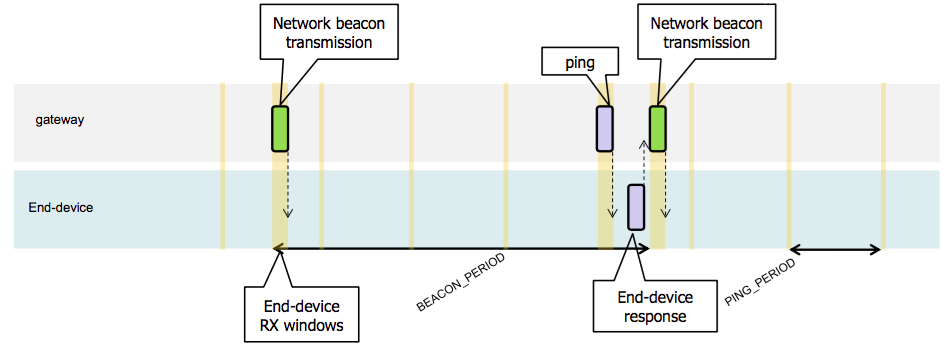
\includegraphics[width=\textwidth]{img/class_b}
\caption{Class B time diagram}
\label{fig:classb}
\end{figure}

All end-devices join the network as Class A, and the decision to switch to Class B must come from the end-device application layer. If so, the LoRaWAN layer searches for a beacon, and if it is found it selects the data rate and the periodicity of the ping slot.

The end-device must periodically transmit an uplink message to update the routing path in the network server. If no beacon is received for a period, it switches back to class A.

\begin{figure}[]
\centering
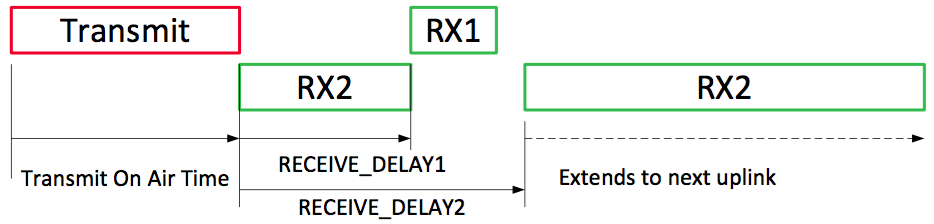
\includegraphics[width=\textwidth]{img/class_c}
\caption{Class C time diagram}
\label{fig:classc}
\end{figure}

Class C is implemented by opening RX2 as often as possible in order to be continuously listening to the channel. This leads to an inefficient protocol, with very high power consumption which is not suitable for battery powered end-devices. Class C end-devices cannot implement Class B option.

\subsubsection{Multicast}
In Class B and Class C mode devices may receive also multicast downlink frames. The \emph{multicast address}, the \emph{NetSessionKey} and the \emph{AppSessionKey} must come from the application layer and multicast frames are not allowed to carry MAC commands. Since ACK are not allowed while operating in multicast mode, the type of the LoRaWAN message must be “Unconfirmed Data Down”.



\section{GWMP: Gateway Message Protocol}
\label{sec:gwmp}
As already stated, each gateway communicates with the network server by means of a standard IP connection. Depending both on the network server and on the packet forwarder installed on the gateway, there can be used different application protocol.

The LoRaWAN specification does not require a specific gateway-to-server protocol, since the server needs to receive the complete LoRa physical payload, encapsulated in the most suitable protocol, depending on specific use case.

However Semtech, the company which has initially developed the LoRa modulation and the LoRaWAN protocol, released also its own gateway-to-server protocol, which is called \emph{Gateway Message Protocol} (GWMP).

GWMP relies on UDP, making it a connection-less protocol, and use the JSON format to carry the received frame with the associated statistics.

\subsection{Message format} Each GWMP message, as its shown in figure \ref{fig:gwmp}, includes three mandatory fields and two optional ones:
\begin{itemize}
\item \emph{Protocol Version}: the version of Gateway Message Protocol used;
\item \emph{Token}: number randomly chosen by the sender to uniquely identify the message;
\item \emph{Type}: it specifies the purpose of the message. Up to version 2 there are six different types defined;
\item \emph{Gateway EUI}: it contains the gateway identifier, based on the EUI-64 specification. It is not present in messages with types PUSH\_ACK or TX\_ACK;
\item \emph{Payload}: it contains a JSON formatted string;
\end{itemize}

\begin{figure}[]
\centering
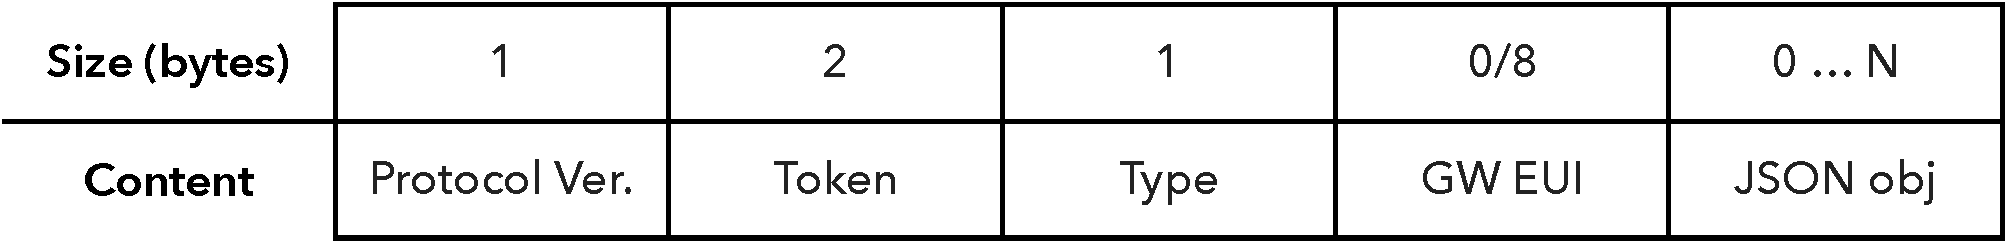
\includegraphics[width=\textwidth]{img/msgformat/gwmp}
\caption{GWMP packet format}
\label{fig:gwmp}
\end{figure}

\subsection{GWMP types}

\begin{itemize}
\item \emph{PUSH\_DATA}: used by the gateway to transmit the network server both the received LoRaWAN frames and other periodic statistics. Its total size shall not exceed 2408 octets;
\item \emph{PUSH\_ACK}: it is transmitted immediately by the network server on a receipt of a PUSH\_DATA message to acknowledge it. It does not contain the gateway EUI and the payload, and the token is the same of the PUSH\_DATA;
\item \emph{PULL\_DATA}: sent periodically by the gateway, it acts as a "keep alive" message informing the network server of the address and UDP port to which send any PULL\_RESP;
\item \emph{PULL\_ACK}: it is transmitted immediately by the network server on a receipt of a PULL\_DATA message to acknowledge it. It does not contain any payload and the token is the same of the PULL\_DATA;
\item \emph{PULL\_RESP}: carries in the JSON object the LoRaWAN frame to transmit to the end-devices and its size shall not exceed 1000 octets;
\item \emph{TX\_ACK}: present only in GWMP version 2, it is used by gateway to acknowledge a PULL\_RESP message.
\end{itemize}
Table \ref{tab:gwmptypes} summarizes all GWMP types;

\begin{table}[]
\centering
\caption{GWMP types}
\label{tab:gwmptypes}
\begin{tabular}{@{}cccc@{}}
\toprule
\multirow{2}{*}{Type} & \multirow{2}{*}{Code} & \multicolumn{2}{c}{Transmitted by} \\
                      &                       & Gateway      & Network Server      \\ \midrule
PUSH\_DATA            & 0x00                  & x            &                     \\
PUSH\_ACK             & 0x01                  &              & x                   \\
PULL\_DATA            & 0x02                  & x            &                     \\
PULL\_ACK             & 0x03                  &              & x                   \\
PULL\_RESP            & 0x04                  &              & x                   \\
TX\_ACK               & 0x05                  & x            &                     \\ \bottomrule
\end{tabular}
\end{table}



\subsection{GWMP Json protocol}
The Json object is used to carry the LoRaWAN messages and other information. To enhance compatibility only ASCII characters are allowed and there must be no white spaces outside the quoted text. Moreover, the top-level JSON object contains other objects as long as they respect the restriction explained above.

\subsubsection{Upstream transmissions}
In upstream transmissions the Json object may contain an array of RXPK objects, one for each LoRa message carried, and one STAT object, which carries some statistics on the gateway.

As already stated, each RXPK object contains a captured LoRa frame, which is encoded in the Base64 format, along with time of receipt and the information of the LoRa channel on which it was detected (data rate, coding rate, frequency, etc.). In listing \ref{list:rxpk} is shown an example of a possible RXPK object.

\begin{lstlisting}[caption={Example of an RXPK object}\label{list:rxpk}]
"rxpk":
[{
	"time":"2013-03-31T16:21:17.528002Z",
	"tmst":3512348611,
	"chan":2,
	"rfch":0,
	"freq":866.349812,
	"stat":1,
	"modu":"LORA",
	"datr":"SF7BW125",
	"codr":"4/6",
	"rssi":-35,
	"lsnr":5.1,
	"size":32, 
	"data":"-DS4CGaDCdG+48eJNM3Vai-zDpsR71Pn9CPA9uCON84"
}]
\end{lstlisting}
The STAT object is used to inform the network server of the status of the gateway. In particular it contains the geographical coordinates of the gateway and the statistics on received and forwarded message. An example of STAT object is reported in listing \ref{list:stat}.

\begin{lstlisting}[caption={Example of an STAT object}\label{list:stat}]
"stat":
{
	"time":"2014-01-12 08:59:28 GMT",
	"lati":46.24000,
	"long":3.25230,
	"alti":145,
	"rxnb":2,
	"rxok":2,
	"rxfw":2,
	"ackr":100.0,
	"dwnb":2, 
	"txnb":2
}
\end{lstlisting}

\subsubsection{Downstream transmissions}
The TXPK object is included in downstream messages to carry the downlink LoRa message along the needed information about the parameters, such as data rate, coding rate and frequency, to use for the transmission. It is important to remark that gateway, in general, do not have any notion about the LoRaWAN layer and its receive windows, so they rely on the time stamp included in the TXPK object to correctly synchronize themselves with the end-devices receive windows. Listing \ref{list:txpk} reports a possible instance of a TXPK object.
\\
\\
\begin{lstlisting}[caption={Example of an TXPK object}\label{list:txpk}]
"txpk":
{
	"imme":true,
	"freq":864.123456,
	"rfch":0,
	"powe":14,
	"modu":"LORA",
	"datr":"SF11BW125",
	"codr":"4/6",
	"ipol":false,
	"size":32,
	"data":"H3P3N2i9qc4yt7rK7ldqoeCVJGBybzPY5h1Dd7P7p8v"
}
\end{lstlisting}

\section{LoRa Servers}
\label{sec:loraservers}
\begin{figure}[]
\centering
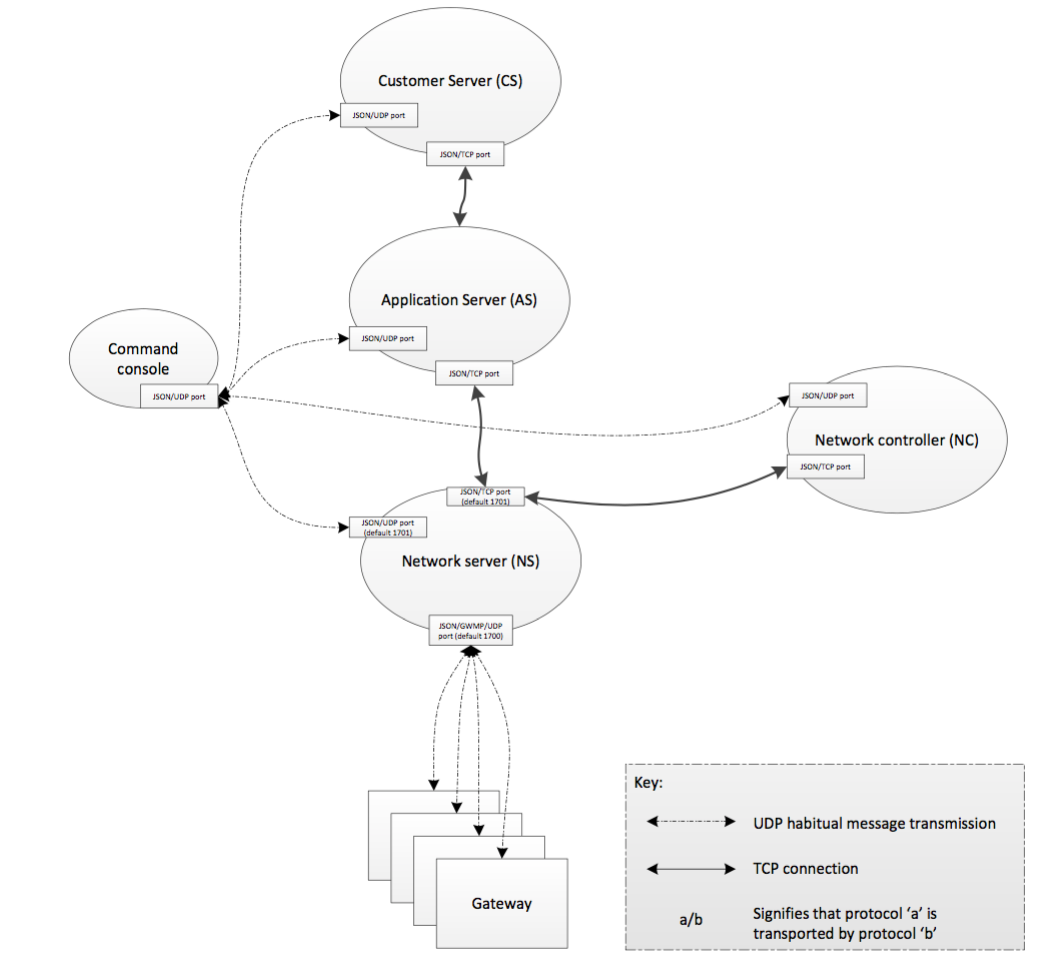
\includegraphics[width=\textwidth]{img/server_flow}
\caption{Architecture of the LoRa servers}
\end{figure}


In the LoRa architecture all the network management is done in the cloud by means of a set of servers. It consists of a \emph{Network Server}, which is responsible for all network management, one or more \emph{Application Server}, which are in charge of handling the end-device join and guarantee the secrecy of the communication. The Application Server may offer an interface to third party software, which in LoRa terminology is called \emph{Customer Server}.
Particularly important is the role played by the \emph{Network Controller}, which is in charge of managing the data rate and RF output for each end-device for which the adaptive data rate (ADR) scheme is enabled.

\subsection{Network Server}

The network server authenticates the received frame and forwards user data to an application server. The received frame is transported from the Gateway to the network server using JSON/GWMP/UDP/IP (defined in section \ref{sec:gwmp}). The frame is forwarded to an application server typically using JSON/TCP/IP.

The network server adds a cryptographic hash to all LoRa frames transmitted to the LoRa end-devices. The hash algorithm is defined by the LoRaWAN specification. \cite{lorawanspec}

A single network server may be connected to many application servers and network controllers. The remote server or controller used for a given mote is determined by the application to which the mote is assigned.

\subsection{Application Server}
The LoRa application server is responsible for admitting Over-The-Air end-devices to the network and for encrypting user data sent to, and decrypting user data received from, the end-device.
A single application server may be connected to many networks and customer servers. The remote server or controller used for a given mote is determined by the application to which the mote is assigned.
The LoRa application server decrypts the received user data and forwards it to a customer server. It also encrypts downstream user data before forwarding it to the network server. The encryption algorithm is defined by the LoRaWAN specification. \cite{lorawanspec}


\subsection{Network Controller}
The network controller receives the transmission parameters used by the mote and characteristics of the signal received by the gateway for each frame. It may perform operations using that data, for instance it may compute some statistics on it in order to find the optimal parameters that maximize the network capacity.
A single network controller may be connected to many network servers. The remote server or controller used for a given mote is determined by the application to which the mote is assigned.


\section{Related work}
The very good performances promised by LoRa, combined with the open specification of the MAC layer, attracted the attention of the scientific community on this technology. 

However the project started only few years ago, so there are not many detailed benchmarks on LoRa. In the following sections some works are reported.

\subsection{Free space measurament}
One of the first performance evaluation was performed in 2014 at the Offenburg University of Applied Sciences, Germany, by the Laboratory Embedded Systems and Communication Electronics. In their experiments they tried to find the maximum distance at which it is possible to transmit in the 868 MHz band with LoRa in free space and line-of-sight conditions.

Using the data rate SF10BW250 and coding rate 4/6 they were able to achieve 100\% of correctly received packets up to 7482 meters, when carrying 10 bytes of physical payload. Then they repeated the same experiment with 50 bytes of physical payload, achieving 94.1\% of correctly received packets at 6667 meters, and 80.33\% of correctly received packets at 7482 meters.\cite{freespace}


\subsection{2.4 GHz experiments for safety applications}
Other experiments were performed at the Offenburg University of Applied Sciences in 2015, focusing on the possible use of LoRa for safety applications. In all the four proposed scenarios only the 2.4 GHz band was tested.

In the first scenario they tried to find how many reinforced walls a LoRa packet could pass through, getting a promising result of 3 walls with 33\% of correctly received packets.

In the second scenario they proved that they need only one LoRa receiver to cover a floor, in comparison with Bluetooth LE which needs four receivers to cover the same area.

In the third scenario they achieved the 81.58\% of correctly received packets at 9.75 Km of distance in a true line-of-sight condition.

In the last scenario they tested the reliability of LoRa in salty water, obtaining 94.5\% of correctly received packets at 2 meters of distance in free space, plus 10 cm of salty water.\cite{safetylora}

\subsection{Wireless image sensor with shared activity time}
The main advantage of transmitting on ISM bands is that they are toll-free, while its disadvantage consists in the strict regulation on it. 

In particular, to overcome the duty cycle limit imposed on the 868 MHz band a french research team at the University of Pau, France, proposed to consider all the individual activity time in a shared/global manner, so that devices that need to go beyond the activity time limitation can borrow activity time from other devices.

This innovative proposal enables multimedia applications, such as image sensor for surveillance purposes, on the low bit rate LoRa network. To effectively share the activity time among the different devices they proposed through which the base station keeps track of the available \emph{Global Activity Time} and broadcasts it to all devices in its network.\cite{imagesensor}
